\chapter{Design of MPI\_T support in CALIPER}

Caliper is an application introspection tool that relies on source code annotations to collect information and perform profiling related tasks. I shall first provide a basic overview of relevant Caliper concepts before describing the MPI\_T support in Caliper. 

\section{Caliper Concepts}
\subsection{Caliper API}
Caliper provides an application level API that acts as the portal for carrying out performance measurements. Caliper also provides high-level annotation macros that are user-friendly. The basic idea behind the source-code annotation API is to associate performance measurements with user-defined, high-level \textit{context information}. These source code annotations act as hooks for background processing. Caliper is built into a library and linked into the application. Figure \ref{fig:caliexample}\footnote{Image taken from: https://llnl.github.io/Caliper} is an example of a Caliper-annotated \verb+C+\texttt{++} source code.
\subsection{Attributes: Caliper's Building Blocks}
Caliper provides a generic \textit{key-value} data model for storing performance data of all kinds. Caliper \textit{attributes} are the basic elements of the Caliper data model. The keys need to have a unique name and a type. They can also optionally have properties which determine how the attributes get processed. An example would be an attribute to track PAPI counters or an attribute to track the total time spent inside a routine or code section. 
\par Among all the properties that an attribute can have, the most important attribute in the context of MPI\_T is the \verb+AS_VALUE+ property. Attributes with the \verb+AS_VALUE+ property set to true cannot be nested. For example, the attribute to track PAPI counters cannot be nested, but the attribute to track the time spent inside a routine is nested.
\begin{center}
	\begin{figure*}[tbp!]
         \centering
		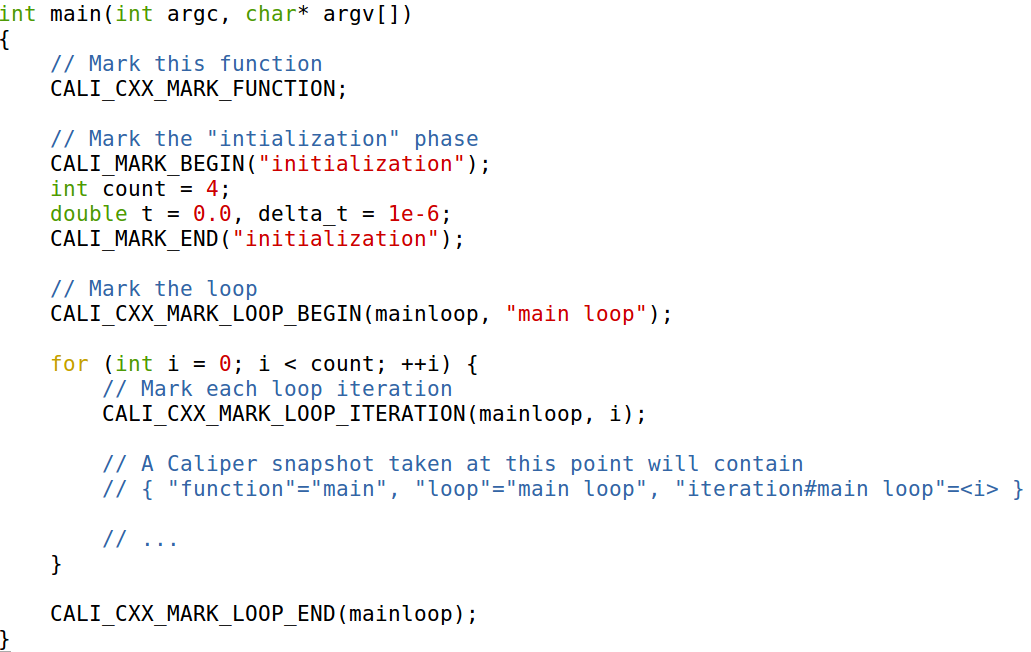
\includegraphics[scale=0.3, width=\columnwidth, keepaspectratio]{figures/cali-example}
		\caption{Caliper~\cite{CALIPER} Annotated Source Code}
		\label{fig:caliexample}
	\end{figure*}
\end{center}
\subsection{Blackboards and Snapshots}
Whenever a performance measurement is made by use of Caliper's measurement API, the values of one or more attributes are updated in an internal data-structure referred to as the \textit{blackboard}. This blackboard is a runtime buffer that is used to combine active attributes, and is updated by Caliper data providers (annotations).
\par A \textit{snapshot} saves the current context of the blackboard. A snapshot can be triggered independently of blackboard updates. Additional information can be added to the snapshot via callbacks to snapshot events. 
\subsection{Services}
Caliper \emph{services} are the basic building blocks that can be combined freely to realize advanced profiling/tracing capabilities. Services are essentially plugins that register callbacks for events of interest. During Caliper initialization, the registered initialization function of each required service is invoked, and the service then performs start-up related tasks inside this initialization function. 
\par An example of a service is the \textit{MPI} service. The MPI service keeps track of the time spent inside MPI calls by utilizing the PMPI interface. The \textit{recorder} service writes Caliper snapshot records into a file using a custom text-based I/O format. The recorder service in conjunction with the MPI service can be used to gather a basic profile of an MPI application. Figure \ref{fig:caliservices} is an illustration of this use case. 
\begin{center}
	\begin{figure*}[bp!]
         \centering
		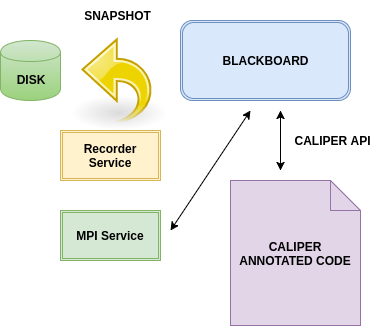
\includegraphics[scale=0.7, keepaspectratio]{figures/cali-services}
		\caption{MPI Profiling: Caliper~\cite{CALIPER} Service Flow}
		\label{fig:caliservices}
	\end{figure*}
\end{center}


\section {MPI\_T Service}
This section describes the design of the MPI\_T service that performs runtime MPI library introspection through the MPI\_T interface. As of the time being, this service does not support performance monitoring or tuning through the MPI\_T interface. 

\section{Creating a performance session}
In order to use MPI\_T, a tool must first create a \emph{performance session} and associate \emph{handles} for the performance variables it wishes to read. Performance sessions allow the MPI library to distinguish between multiple tools / software modules that may be simultaneously querying the MPI\_T interface. \\
The \emph{MPIT} Caliper service creates an MPI\_T performance session during the Caliper service registration phase.
\section{PVAR handle allocation}
Before a tool can read the value of a PVAR, it must first allocate a \emph{handle} for the PVAR. The MPI\_T interface specifies a function that allows a tool to know the number of PVARs exported by an MPI implementation at any given point in time. A couple of points need to be kept in mind when allocating PVAR handles:
\begin{itemize}
	\item Number of PVARs can change: The number of PVARs exported by the library can change at any point in time. Typically, MPI libraries export additional PVARs after \verb+MPI_Init+. Caliper allocates handles for PVARs from multiple places: During the registration for the \emph{MPIT} service, inside the wrapper for \verb+MPI_Init+, and from inside the wrapper for certain MPI calls (description follows).
	\item PVARs can be bound to MPI objects: The \verb+MPI_pvar_get_info+ function returns the \emph{bind} type for the PVAR. The idea here is that PVARs can be \emph{associated} with a specific object such as a communicator or message. As a result, there can be multiple handles allocated for a PVAR at any given index. These handles must be allocated appropriately depending on the bind type.
		\begin{itemize}
			\item \verb+MPI_T_BIND_NO_OBJECT+: These PVARs are not bound to any MPI object --- Caliper allocates handles for such PVARs during Caliper registration and inside the wrapper for \verb+MPI_Init+.
			\item \verb+MPI_T_BIND_MPI_COMM+: These PVARs are bound to MPI communicators, and is a special case. Handles for pvars bound to \verb+MPI_COMM_WORLD+ and \verb+MPI_COMM_SELF+ are allocated during Caliper registration phase. Additionally, handles are created each time \verb+MPI_Comm_create+ is invoked, by intercepting the call through the PMPI wrapper.
			\item \verb+MPI_T_BIND_WIN+: These PVARs are bound to MPI windows. As a result, handles for such pvars are allocated inside the Caliper PMPI wrapper for \verb+MPI_Win_create+.
			\item \verb+MPI_T_BIND_MPI_ERR_HANDLER+: These PVARs are bound to MPI error handlers. Handles for such pvars are allocated inside the PMPI wrapper for \verb+MPI_Errhandler_create+.
			\item \verb+MPI_T_BIND_MPI_FILE+: These PVARs are bound to file objects. Handles are allocated inside the PMPI wrapper for \verb+MPI_File_open+.
			\item \verb+MPI_T_BIND_MPI_GROUP+: These PVARs are bound to MPI group objects. Handles are allocated inside the PMPI wrapper for \verb+MPI_COMM_GROUP+.
			\item \verb+MPI_T_BIND_MPI_OP+: These PVARs are bound to MPI reduction operators. Handles are allocated inside the PMPI wrapper for \verb+MPI_Op_create+.
			\item \verb+MPI_T_BIND_MPI_INFO+: These PVARs are bound to MPI Info objects. Handles are allocated inside the PMPI wrapper for \verb+MPI_Info_create+.
			\item \verb+MPI_T_BIND_MPI_MESSAGE+, \verb+MPI_T_BIND_MPI_REQUEST+: Not supported inside Caliper currently. Open question --- how do we allocate handles for these?
		\end{itemize}
\end{itemize}
\section{PVAR classes and notion of aggregability}
Depending on what they represent, PVARs are categorized into counters, state variables, watermarks, etc., and are handled differently. For this purpose, we define the notion of aggregatability as follows: Any PVAR on which it is \emph{meaningful} to apply one or more of (SUM, MAX, MIN, AVG, COUNT) operators is defined as aggregatable.\\
Along with other information, a call to \verb+MPIT_pvar_get_info+ returns the \emph{CLASS} to which the PVAR belongs. The various classes, along with how Caliper handles them are:
\begin{itemize}
	\item \verb+MPI_T_PVAR_CLASS_TIMER+, \verb+MPI_T_PVAR_CLASS_AGGREGATE+, \\\verb+MPI_T_PVAR_CLASS_COUNTERS+: These are free-counting, monotonically increasing values. As such, they are not aggregatable, but by storing the "last" value for these counters and timers, the difference between the current and last value is a derived metric that is aggregatable by use of \emph{SUM}, \emph{MAX}, \emph{MIN}, \emph{AVG} operators. Storing this difference is more useful than just the raw counter values, as one would typically by interested in the \emph{change} caused to any of these PVARs rather than the raw value itself.
	\item \verb+MPI_T_PVAR_CLASS_STATE+: Represents MPI state at any instant in time. Non-aggregatable value.
	\item \verb+MPI_T_PVAR_CLASS_SIZE+: Represents size of an MPI resource. Non-aggregatable value.
	\item \verb+MPI_T_PVAR_CLASS_LEVEL+, \verb+MPI_T_PVAR_CLASS_PERCENTAGE+: Represents the instantaneous level or percentage utilization of an MPI resource. It is meaningful to apply the \emph{AVG}, \emph{MIN}, \emph{MAX} operators, and hence these classes are aggregatable.
	\item \verb+MPI_T_PVAR_CLASS_HIGHWATERMARK+, \\\verb+MPI_T_PVAR_CLASS_LOWWATERMARK+: As such, they are non-aggregatable. However, one can define aggregatable derived metrics out of these PVARs. Specifically, Caliper defines two derived metrics: A boolean that tells us if the watermark has gone up from the last time it was read, and a double value specifying the \emph{change} in the value between successive reads. Both of these derived metrics are aggregatable quantities as one can apply the \emph{COUNT} and / or \emph{SUM} operator to them.
	\item \verb+MPI_T_PVAR_CLASS_GENERIC+: Represents PVARs that do not fall into any of the above classes. These PVARs would need to handled on a case-by-case basis, and thus for now, we define these as non-aggregatable values.
\end{itemize}

\section{Creating Caliper attributes for PVARs}
The basic data unit in Caliper is an attribute. An attribute is a key value pair that has certain properties. For each PVAR exposed by the MPI library, Caliper defines an attribute with the same name as the PVAR. Each PVAR attribute has the following properties:
\begin{itemize}
	\item \verb+CALI_ATTR_AS_VALUE+ - We do not want "stacking" for PVAR values. They should be treated much the same way as PAPI counters.
	\item \verb+CALI_ATTR_SCOPE_PROCESS+ - PVARs are defined on a per-rank basis
	\item \verb+CALI_ATTR_SKIP_EVENTS+ - We do not want callbacks to be triggered everytime the attribute for a PVAR is updated
	\item \verb+Metadata (class.aggregatable)+ - Boolean value specifying if the PVAR is aggregatable or not. Aggregatability is determined in accordance with the rules above. 
\end{itemize}
Apart from creating a Caliper attribute for each PVAR exported, there are two additional attributes created for each watermark PVAR exported --- one that represents the number of times the watermark changes, and another that represents the cumulative change in the watermark PVAR. 

\section{Querying and storing PVARs}
In the current design, all PVARs exported by the MPI library are queried when a snapshot is triggered. By integrating the \emph{MPIT} service along with the \emph{MPI} service, this would be useful in determining how various MPI function calls contribute to changes in PVAR values. Moreover, one can gather meaningful information by aggregating using MPI function names or annotated code regions as keys. Currently, we note about 10-15\% overheads in collecting PVARs during every snapshot event. This may not be a very scalable option, as this overhead would increase with a rise in number of PVARs exported.\\
Depending on the class of the PVAR, we either store the raw value read from the interface in the snapshot, or a derived metric.
\begin{itemize}
	\item \verb+MPI_T_PVAR_CLASS_TIMER+, \verb+MPI_T_PVAR_CLASS_AGGREGATE+, \\\verb+MPI_T_PVAR_CLASS_COUNTERS+: We store the difference between the current value and the "last value" for such PVARs in the snapshot. Storing and aggregating this derived value is more meaningful --- it helps us answer questions such as: How do different MPI functions contribute to this PVAR? Which MPI function is responsible for the highest value?
	\item \verb+MPI_T_PVAR_CLASS_STATE+, \verb+MPI_T_PVAR_CLASS_SIZE+: These PVARs are stored as is in the snapshot. Perhaps it may be more meaningful to view changes \emph{over time}, such as in a trace.
	\item \verb+MPI_T_PVAR_CLASS_HIGHWATERMARK+, \verb+MPI_T_PVAR_CLASS_LOWWATERMARK+: Along with storing the raw value for watermark PVARs, we store the derived metrics that represent the number of times the watermark changed, along with how much the watermark changed in the snapshot. By aggregating across MPI functions for example, we can answer questions such as: Which function most frequently pushed up / down a watermark? Which function was responsible for the highest cumulative change in a given watermark?
	\item \verb+MPI_T_PVAR_CLASS_LEVEL+, \verb+MPI_T_PVAR_CLASS_PERCENTAGE+: We store these PVARs as is in the snapshot. It maybe meaningful to view the average, maximum or minimum value for these PVARs, aggregated across MPI functions.
\end{itemize}

\section {Challenges in implementing MPI\_T in Caliper}
Use the LLNL slide info.

